% Gemini theme

\documentclass[final]{beamer}
\usepackage{biblatex}

\addbibresource{poster.bib}

% ====================
% Packages
% ====================

\usepackage[T1]{fontenc}
%\usepackage{sectsty}
%\renewcommand{\familydefault}{sectsty}
\usepackage{bold-extra}



\usepackage{lmodern}
\usepackage[size=custom,width=90,height=70,scale=1.0]{beamerposter}
\usetheme{gemini}
\usecolortheme{uchicago}
\usepackage{graphicx}
\usepackage{booktabs}
\usepackage{tikz}
\usepackage{pgfplots}
\pgfplotsset{compat=1.17}

\usepackage[justification=justified,
  format=plain]{caption}
   
\usepackage{fancyvrb}

% ====================
% Lengths
% ====================

% If you have N columns, choose \sepwidth and \colwidth such that
% (N+1)*\sepwidth + N*\colwidth = \paperwidth
\newlength{\sepwidth}
\newlength{\colwidth}
\setlength{\sepwidth}{0.025\paperwidth}
\setlength{\colwidth}{0.3\paperwidth}

\newcommand{\separatorcolumn}{\begin{column}{\sepwidth}\end{column}}

% % ====================
% % Title
% % ====================

\title{\fontsize{65}{0}\selectfont Bi-variate TrendCalculus on Financial Streams}

\author{\fontsize{30pt}{20pt}\selectfont Virginia Jimenez Mohedano \and Stavroula Rafailia Vlachou \\
\vspace*{0.2in}
\fontsize{25pt}{20pt}\selectfont Supervisor: Raazesh Sainudiin}
%\vspace*{-0.1in}


% % ====================
% % Footer (optional)
% % ====================

\footercontent{
  \href{mailto:virginia.jimenezmohedano.6097@student.uu.se}{virginia.jimenezmohedano.6097@student.uu.se} \hfill
  Project in Data Science \hfill
  \href{mailto:stavroula.vlachou.2231@student.uu.se}{stavroula.vlachou.2231@student.uu.se}}
% (can be left out to remove footer)

% ====================
% Logo (optional)
% ====================

% use this to include logos on the left and/or right side of the header:
%\logoright{\includegraphics[height=7cm]{logos/UU_logo_2färg.eps}}
\logoleft{
\includegraphics{logos/UU_logo_vit.eps}}

% ====================
% Body
% ====================

\begin{document}
\begin{frame}[fragile]
\begin{columns}[t]
\separatorcolumn

\begin{column}{\colwidth}

  \begin{block}{Introduction}
    This project amounts to identifying \textsf{\textbf{long term trends}} on financial time series from historical data and it is an attempt towards performing a scalable data science pipeline for \textsf{\textbf{causal inference}} on trend change events of high order. 
  \end{block}
  
  \begin{block}{Approach}
  For the analysis the following tools and frameworks were utilized:
    \begin{enumerate}
        \item Historical data of financial time series \cite{HistData}.
        \item Apache Spark ecosystem to handle the big volume of the data. 
        \item TrendCalculus algorithm \cite{TrendCalculus} to identify long term trends.
        \item Pathogen algorithm \cite{Pathogen} to establish causal inference between events of two or more time series. 
    \end{enumerate}
  \end{block}

    \begin{block}{Methods}
      \vspace{0.6in}
      \begin{figure}
         \centering
         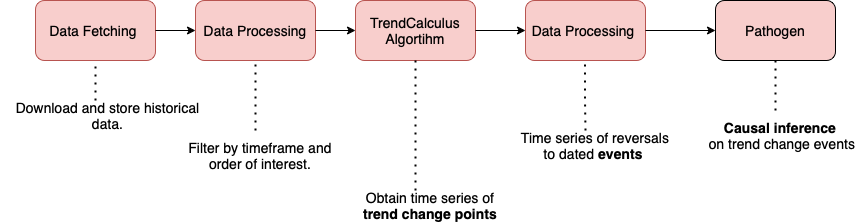
\includegraphics[width=1\textwidth]{Pipeline.png}
         \caption{Summary of the main levels of the pipeline}
         \label{fig:my_label}
      \end{figure}
      \textsf{\textbf{Data:}} Historical data from the foreign exchange market for the trading of currencies. The data sets consist of pairs of currencies and futures/commodities with \textsf{\textbf{values}} recorded \textsf{\textbf{every one minute}} over the last two decades.\\
      \vspace{0.6in}
      \textsf{\textbf{Cloud Computing:}} A cluster was utilized in order to distribute the computational tasks and scale on demand within the Apache Spark framework.\\
      \vspace{0.6in}
      \textsf{\textbf{Long term trends:}} The TrendCalculus algorithm provided an efficient solution on establishing high order trend change points.\\
      \vspace{0.6in}
      \textsf{\textbf{Causal inference:}} The returned time series was encoded to be suitable as input to Pathogen by turning consecutive  $n$-th order reversals to events.\\
     \end{block}
    \vspace{0.5in}
    
     \begin{alertblock}{}
      Our project work is available as examples and notebooks at \cite{TrendCalculusNotebooks} and \cite{PathogenNotebooks}.  
     \end{alertblock}

\end{column}

\separatorcolumn



\begin{column}{\colwidth}
%\vspace{1in}
    \begin{block}{TrendCalculus}
        
    \begin{itemize}
    \item Stream the data across a fixed window size. 
    \item For each window identify the dated High and Low. 
    \item Summarise each window as rising or falling.
    \item Compare the summary of the current window to the previous one. 
    \item Assign a sign for each window according to the TrendCalculus equation \ref{TrendCalculusEquasion}. 
    \end{itemize}
    \begin{equation}\label{TrendCalculusEquasion}
        sign(sign(H_{p_i}-H_{p_{i-1}})+sign(L_{p_i}-L_{p_{i-1}}))
    \end{equation} 
    where 
    \begin{itemize}
        \item H, L $=$ High, Low
        \item $p_i=$ current window,\hspace{0.4cm} $p_{i-1}=$ previous window
    \end{itemize}
   Output: A time series of trend change points - \textsf{\textbf{reversals}}. The latter can be used as input to the algorithm iteratively to find reversals of higher order and establish long term trends.
   \end{block}
   
   \begin{block}{Showcase}
  \begin{itemize}
      \item \textsf{\textbf{Gold}} is usually seen as an \textsf{\textbf{hedge against inflation}} by investors. \item \textsf{\textbf{Increasing oil prices}} can lead to inflation.
  \end{itemize}
  \textsf{\textbf{Can a change in oil price be a predictor of a change in gold price?}}
  \vspace{-1.25in}
  \begin{figure}[h!]
      \centering
      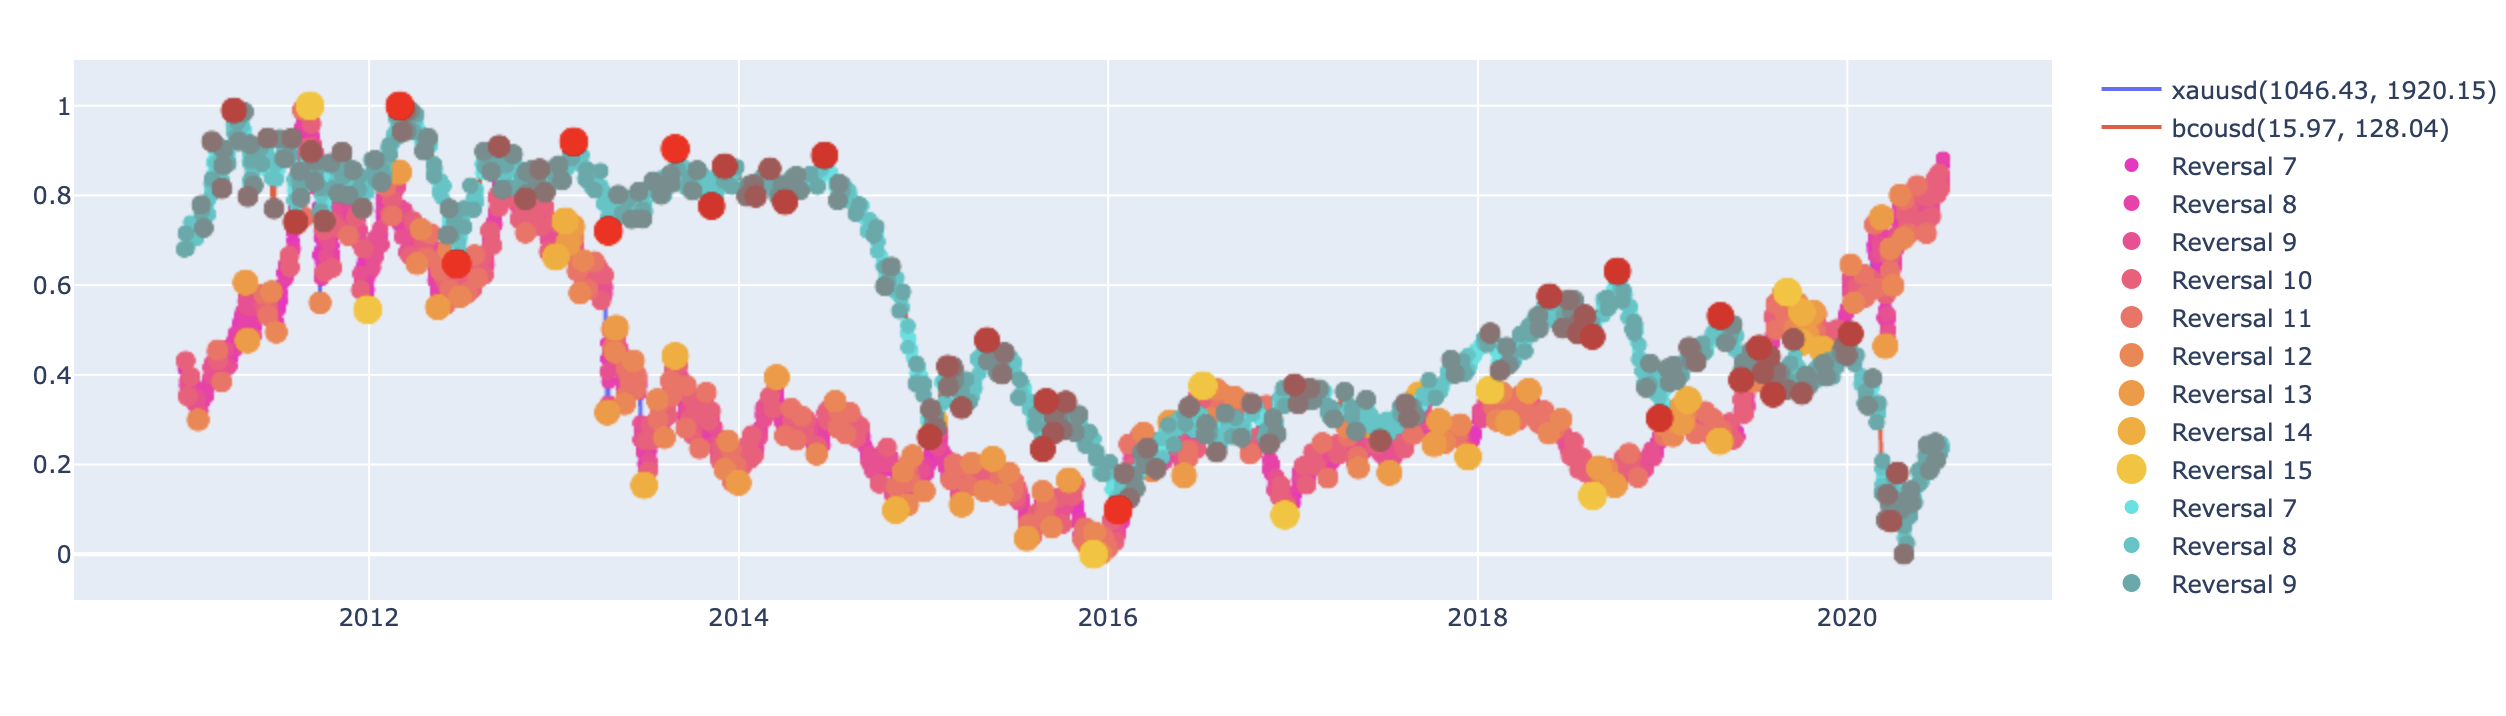
\includegraphics[width=1.05\textwidth]{GoldOil.png}
      \vspace{-0.8in}
      \caption{Output of TrendCalculus on Gold price and Brent Crude Oil price in USD. The reversals of each time series are illustrated as spheres whose radius and color intensity are proportional to the reversal order.}
      \label{fig:GoldOil}
  \end{figure}
  \textsf{\textit{Gold prices tend to move up and down in tandem with oil prices.}}
  \end{block}
   
   
   \begin{block}{Encoding the ID}
The occurrence of consecutive reversal points for a specific reversal order is turned into \textsf{\textbf{events}}. Each event is associated with an id.


\begin{figure}
\begin{BVerbatim}[baselinestretch=0.1,fontsize=\small]

+------------+--------------------+-----------+-----------------+

| MaxRev = 7 | Time series id = 1 | Trend = 1 | Slope value = 2 |

+------------+--------------------+-----------+-----------------+

\end{BVerbatim}
    
\caption{Example of the encoding for the event with id 7112. The MaxRev attribute stands for the reversal order, the Time series id is 1 for the Oil time series and 2 for the Gold, the Trend is 0 for a falling trend and 1 for a rising trend and the Slope value is the normalized slope of the event values.}
\label{fig:ID}
 \end{figure}

\end{block}
\end{column}
\separatorcolumn



\begin{column}{\colwidth}

  \begin{block}{Extensions - Pathogen}
    \begin{itemize}
        \item Observe a true causation signal on time related events (by generating random correlations over the same events at different times).
        \item Output the causal effects structured as a graph (observed and normalized correlations).
        \item Extract the most probable causes and effects by returning a graph where the vertices contain the score of two \textsf{\textbf{measures}}:\newline
        \begin{itemize}
            \item \textsf{\textbf{Aggressiveness}}: how likely an event could explain downstream effects.
            \vspace{0.3in}
            \item \textsf{\textbf{Sensitivity}}: how likely an event results from an upstream event cause.

        \end{itemize}   
    \end{itemize}
\vspace*{-0.3in}
\begin{figure}
\begin{BVerbatim}[fontsize=\small]
+-----+-----+------------------+--------------------+--------------------+
|  src|  dst|          normCorr|      aggressiveness|         sensitivity|
+-----+-----+------------------+--------------------+--------------------+
| 7210|61014|0.9259259259259258| 0.14875136530932828|0.019126830444798487|
| 7210|61113|0.8064516129032259| 0.14875136530932828|0.016698026578792328|
+-----+-----+------------------+--------------------+--------------------+
\end{BVerbatim}
\caption{Output of Pathogen: The src and dst indicate the event id's of the related nodes, the normCorr stands for the normalized correlation and the last two arguments are the causality measures mentioned above. The event 7210, i.e., a small rise in gold price at order 7, seems to precede both 61014 and 61113, which are order 6 oil price fall and rise of fairly steep normalised slopes. In other words, there is strong evidence for a slight rise in gold price seeming to just precede a rather sharp fall or rise in the oil price at orders 6 and 7, respectively.
}
\label{fig:data_pathogen}
\end{figure}
\end{block}

\begin{block}{Discussion and Conclusions}
    The TrendCalculus algorithm provides a  powerful solution for identifying major trend change points in an efficient manner.
    Notably, the implementation is not limited to financial time series, but rather can receive as input any time series. In addition, Pathogen seems to capture part of our intuition regarding the co-movement of Gold and Oil prices.
    
    We believe that the combination of the two algorithms that have the distinguishing feature of being able to scale to arbitrarily large data sets can be very beneficial for discovering causal inference among multivariate time series.  
\end{block}



\begin{block}{Acknowledgments}
\fontsize{20}{10}\selectfont This project was supported by Combient Mix AB through Data Science Project Fellowships between 2021-10 and 2021-12 to Stavroula Rafailia Vlachou and Virginia Jimenez Mohedano at Combient Competence Centre for Data Engineering Sciences, Department of Mathematics, Uppsala University, Uppsala, Sweden, and Databricks University Alliance with infrastructure credits from AWS.\\
Many thanks to Andrew Morgan and Antoine Amend for their guidance.
\end{block}


\begin{block}{References}
    \nocite{*}
    
    \AtNextBibliography{\fontsize{15}{10}\selectfont} 
    \printbibliography
    

  \end{block}
\vspace{-0.1in}

\end{column}
\separatorcolumn

%   \begin{block}{Bibliography}
% \nocite{*}
% \printbibliography
% \end{block}
\end{columns}
\end{frame}

\end{document}
